\documentclass[12pt]{exam}

\newcommand{\course}{MTH 234 Summer 2021}
\newcommand{\qdate}{16.1-2 Vector Fields and Line Integrals} %PUT DATE HERE
\newcommand{\quiz}{Group Work} 

    \usepackage[top=1in, bottom=1in, left=.45in, right=.45in]{geometry}
    \usepackage{amsmath,amsthm,amssymb,amstext}
    \usepackage{enumerate,enumitem}
    \usepackage{tikz,float,graphicx}
    \usepackage{microtype}
    \usepackage{bm,tikz}
        \usetikzlibrary{calc}
    \usepackage{multicol}
    \usepackage{nicematrix}
    \usepackage{cleveref}
    \usepackage[framemethod=tikz]{mdframed}
    
    %\newcommand{\course}{MTH 234 Summer 2021}
    %\newcommand{\qdate}{Equations of lines and planes} %PUT DATE HERE
    %\newcommand{\quiz}{Group Work} 
    
    \newcommand{\R}{\mathbb{R}}
    
    \newcommand{\ba}{\bm{a}}
    \newcommand{\bb}{\bm{b}}
    \newcommand{\bc}{\bm{c}}
    \newcommand{\bi}{\bm{i}}
    \newcommand{\bj}{\bm{j}}
    \newcommand{\bk}{\bm{k}}
    \newcommand{\br}{\bm{r}}
    \newcommand{\bv}{\bm{v}}
    \newcommand{\gen}[1]{\left\langle #1 \right\rangle}

\newtheorem*{theorem}{Theorem}
\surroundwithmdframed[]{theorem}

\theoremstyle{definition}
    \newtheorem*{definition}{Definition}
    \surroundwithmdframed[]{definition}
    \newtheorem*{info}{Useful Information}
    \surroundwithmdframed[]{info}
\theoremstyle{remark}
    \newtheorem*{remark}{Remark}
    \surroundwithmdframed[]{remark}
    

%%%%%%%%%%%%%%%%%%%%%%%
% HEADER AND FOOTER
%%%%%%%%%%%%%%%%%%%%%%%
\pagestyle{headandfoot}
\firstpageheadrule
\runningheadrule
\firstpageheader{\course}{\quiz}{\qdate}
\runningheader{\course}{\quiz}{\qdate}
\runningfooter{}{}{}


\usepackage{color}
\shadedsolutions
\definecolor{SolutionColor}{rgb}{0.8,0.9,1}

\usepackage{pgfplots}
    \pgfplotsset{every axis/.append style={
                    axis x line=middle,    % put the x axis in the middle
                    axis y line=middle,    % put the y axis in the middle
                    axis line style={<->}, % arrows on the axis
                    xlabel={$x$},          % default put x on x-axis
                    ylabel={$y$},          % default put y on y-axis
                    grid=both,
                    %xtick={-4,...,-1,1,...,3},
                    %ytick={-1,1,}
    }}
    \pgfplotsset{compat=1.17}

\newcommand{\bif}{\quad\iff\quad}

\printanswers
%\noprintanswers

\begin{document}

\subsection*{Vector Fields}

\begin{questions}

\question Sketch the vector field \(\bm{F}(x,y)=\gen{y,x}\).
\ifprintanswers
    \begin{solution}
    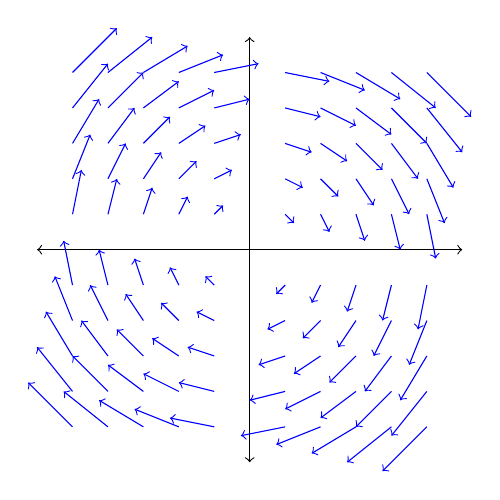
\begin{tikzpicture}[scale=.9]
        \draw[thin,<->] (-3,0)--(3,0);
        \draw[thin,<->] (0,3)--(0,-3);

        \foreach \x in {-2.5,-2,-1.5,-1,-0.5,0.5,1,1.5,2,2.5}
        {
            \foreach \y in {-2.5,-2,-1.5,-1,-0.5,0.5,1,1.5,2,2.5}
            {
                \draw[->,blue] (\x,\y) -- ++(0.25*\y,-0.25*\x);
            }
        }
    \end{tikzpicture}
    \end{solution}
    \else
        \vfill
    \fi

\question Match the vector fields \(\bm{F}\) with their plots

\begin{minipage}[t]{0.3\textwidth}
\begin{parts}
    \part \(\bm{F}(x,y)=\gen{x,-y} \)
    \ifprintanswers
        \begin{solution}
        A
        \end{solution}
    \else
        \vfill
    \fi
    \part \(\bm{F}(x,y)=\gen{-x,y} \)
    \ifprintanswers
        \begin{solution}
        C
        \end{solution}
    \else
        \vfill
    \fi
    \part \(\bm{F}(x,y)=\gen{x,x-y} \)
    \ifprintanswers
        \begin{solution}
        B
        \end{solution}
    \else
        \vfill
    \fi
    \part \(\bm{F}(x,y)=\gen{1,x+y} \)
    \ifprintanswers
        \begin{solution}
        D
        \end{solution}
    \else
        \vfill
    \fi 
\end{parts}
\end{minipage}
\begin{minipage}[t]{0.6\textwidth}
\begin{center}
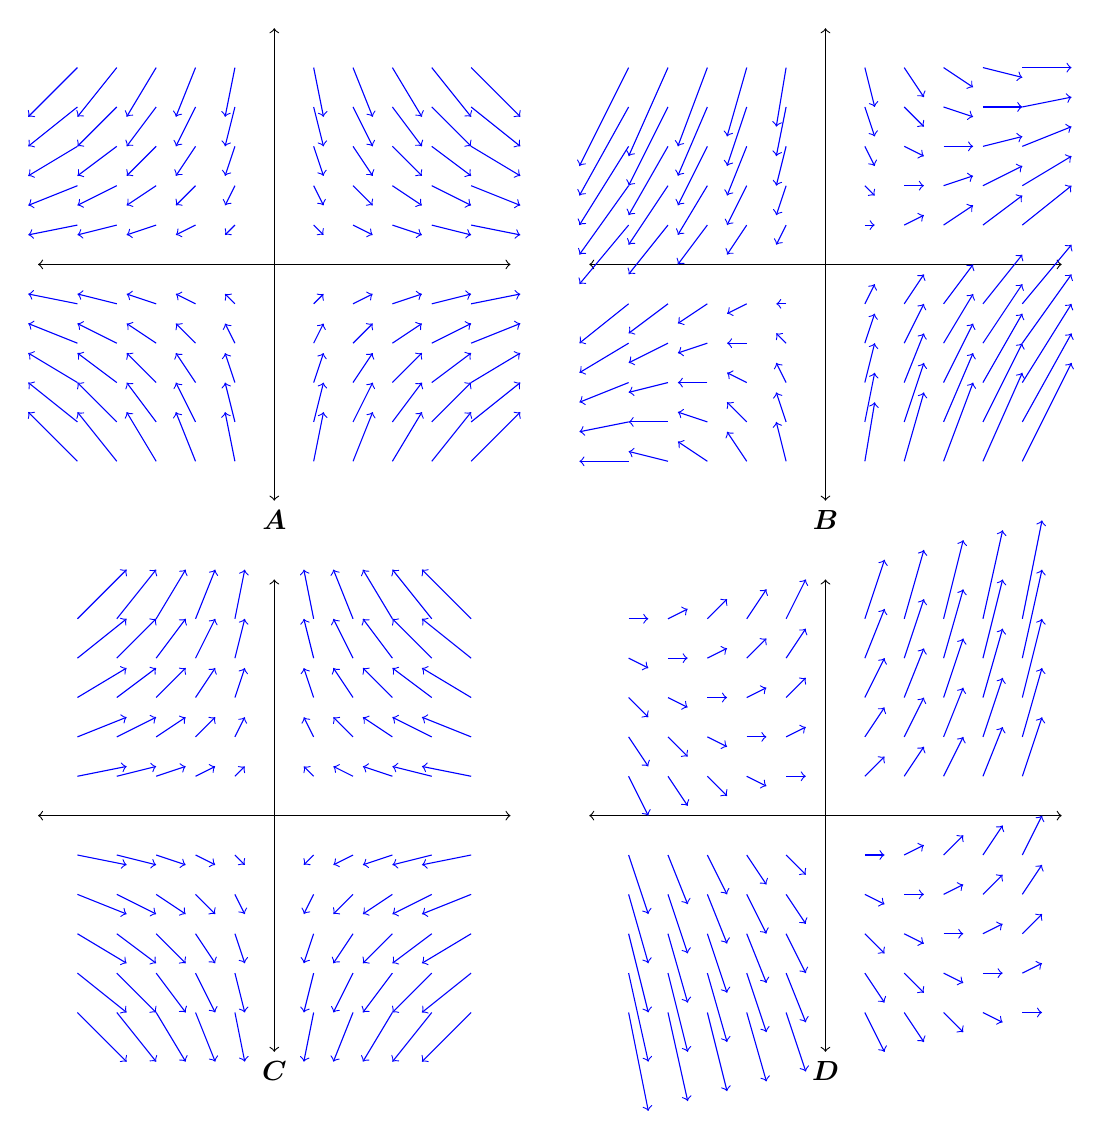
\begin{tikzpicture}
    \begin{scope}
        \draw[thin,<->] (-3,0)--(3,0);
        \draw[thin,<->] (0,3)--(0,-3) node[below] {$\bm{A}$};

        \foreach \x in {-2.5,-2,-1.5,-1,-0.5,0.5,1,1.5,2,2.5}
        {
            \foreach \y in {-2.5,-2,-1.5,-1,-0.5,0.5,1,1.5,2,2.5}
            {
                \draw[->,blue] (\x,\y) -- ++(0.25*\x,-0.25*\y);
            }
        }
    \end{scope}

    \begin{scope}[shift={(7,0)}]
        \draw[thin,<->] (-3,0)--(3,0);
        \draw[thin,<->] (0,3)--(0,-3) node[below] {$\bm{B}$};

        \foreach \x in {-2.5,-2,-1.5,-1,-0.5,0.5,1,1.5,2,2.5}
        {
            \foreach \y in {-2.5,-2,-1.5,-1,-0.5,0.5,1,1.5,2,2.5}
            {
                \draw[blue,->] (\x,\y) -- ++(0.25*\x,0.25*\x-0.25*\y);
            }
        }
    \end{scope}

    \begin{scope}[shift={(0,-7)}]
        \draw[thin,<->] (-3,0)--(3,0);
        \draw[thin,<->] (0,3)--(0,-3) node[below] {$\bm{C}$};

        \foreach \x in {-2.5,-2,-1.5,-1,-0.5,0.5,1,1.5,2,2.5}
        {
            \foreach \y in {-2.5,-2,-1.5,-1,-0.5,0.5,1,1.5,2,2.5}
            {
                \draw[->,blue] (\x,\y) -- ++(-0.25*\x,0.25*\y);
            }
        }
    \end{scope}

    \begin{scope}[shift={(7,-7)}]
        \draw[thin,<->] (-3,0)--(3,0);
        \draw[thin,<->] (0,3)--(0,-3) node[below] {$\bm{D}$};

        \foreach \x in {-2.5,-2,-1.5,-1,-0.5,0.5,1,1.5,2,2.5}
        {
            \foreach \y in {-2.5,-2,-1.5,-1,-0.5,0.5,1,1.5,2,2.5}
            {
                \draw[->,blue] (\x,\y) -- ++(0.25,0.25*(\x+\y);g
            }
        }
    \end{scope}
\end{tikzpicture}
\end{center}
\end{minipage}

\newpage

 \subsection*{Line Integrals}

 \question Evaluate \(\int_{C}y^3~ds\) where \(C\) is the curve \(x=t^3,y=t\) with \(0\le t \le 2\).
 \ifprintanswers
        \begin{solution}
            \begin{align*} 
                \int_0^2 (y(t))^3\sqrt{x'(t)^2+y'(t)^2}dt & = \int_{0}^2 t^3\sqrt{(3t^2)^2+1^2}dt\\
                    & = \int_0^2 t^3\sqrt{9t^4+1}dt\\
                    & = \frac{1}{54}(9t^4+1)^{3/2}|_0^2
                    & = \frac{1}{54}(145)^{3/2}-1)
            \end{align*}
        \end{solution}
    \else
        \vfill
    \fi

 \question Evaluate 
 \[
    \int_{C}(x+2y)~dx+x^2~dy,
 \] where \(C\) is the curve consisting of line segments from \((0,0)\) to \((2,1)\) and from \((2,1)\) to \((3,0)\).
 \ifprintanswers
        \begin{solution}
        First we compute the line integral along \(C_1\) from \(0,0\) to \((2,1)\) parameterized by \(x=2t,y=t\) with \(0\le t \le 1\).
            \begin{align*}
                \int_{0}^1(2t+2t)2+(2t)^2 ~dt & = 4t^2+\frac{4}{3}t^3|_0^1\\
                    & = 4+4/3.
            \end{align*}
            Now along \(C_2\) from \((2,1)\) to \((3,0)\) parameterized by \(x(t)=2+t\), \(y(t)=1-t\) with \(0\le  t\le 1\).
            \begin{align*}
                \int_{0}^1 (2+t+2(1-t))+(2+t)^2(-1)~dt & = \int_0^1 4-t-(t^2+4t+4) dt\\
                    & = \int_0^1 -t^2-5t dt\\
                    & = -\frac{1}{3}t^3-\frac{5}{2}t^2|_0^1\\
                    & = -\frac{1}{3}-\frac{5}{2}
            \end{align*}

            So in total, 
            \[
                \int_{C}(x+2y)~dx+x^2~dy = 4+4/3-1/3-5/2 = 5/2.
            \] 
        \end{solution}
    \else
        \vfill
        \newpage
    \fi

 \question Find the work done by the force field \(F(x,y,z)=\gen{x-y^2,y-z^2,z-x^2}\) on a particle that moves along the line segment from 
 \((0,0,1)\) to \((2,1,0)\).
 \ifprintanswers
        \begin{solution}
            If \(\br(t)=\gen{2t,t,1-t}\), \(0\le t \le 1\), then 
            \begin{align*}
                \int_{0}^1 F(\br(t))\cdot \br'(t) dt & = \int_0^1 \gen{2t-t^2,t-(1-t)^2,1-t-(2t)^2}\cdot \gen{2,1,-1} dt\\
                & = \int_0^1 t^2+8t-2 dt\\
                & = \frac{1}{3}t^3+4t^2-2t|_0^1\\
                & = \frac{7}{3}.
            \end{align*}
        \end{solution}
    \else
        \vfill
    \fi 

 \question Find the work done by the force field \(F(x,y)=x\bi +(y+2)\bj\) in moving an object along an arch of the cyloid 
 \(r(t)=(t-\sin t)\bi +(1-\cos t)\bj\), \(0\le t \le 2\pi\).
 \ifprintanswers
        \begin{solution}
            \begin{align*}
                \int_{0}^{2\pi} \gen{t-\sin t,1-\cos t+2}\cdot\gen{1-\cos t,\sin t} ~dt 
                    & = \int_{0}^{2\pi} (t-\sin t)(1 - \cos t)+(1-\cos t+2)(\sin t)~dt\\
                    & = \int_{0}^{2\pi} t-t\cos(t)+2\sin(t)~dt\\
                    & = \frac{1}{2}t^2-(\cos(t)+t\sin(t))-2\cos(t)|_0^{2\pi}\\
                    & = \frac{1}{2}(2\pi)^2-(1+0)-2(1)-\left(0-(1+0)-2 \right)\\
                    & = 2\pi^2
            \end{align*}
        \end{solution}
    \else
        \vfill
    \fi

\end{questions}

\end{document}

%soln : Question environment
    \ifprintanswers
        \begin{solution}
        \end{solution}
    \else
        \vfill
    \fi